\documentclass[11pt,a4paper]{article}

\usepackage[main=italian,provide=*]{babel}
\usepackage{amsmath,amssymb,mathtools}
\usepackage{tikz}
\usepackage{pgfplots}
\pgfplotsset{compat=1.18}
\usetikzlibrary{arrows.meta,positioning,calc}
\usepackage{booktabs}
\usepackage{colortbl}
\usepackage{capt-of}
\usepackage{geometry}
\geometry{margin=2.6cm}
\usepackage{enumitem}
\usepackage{xcolor}
\usepackage{mdframed}
\usepackage{fancyhdr}

\newcommand{\ket}[1]{\lvert #1\rangle}
\newcommand{\bra}[1]{\langle #1\rvert}
\newcommand{\braket}[2]{\langle #1 \vert #2\rangle}
\newcommand{\vs}[1]{\mathbf{s}_{#1}}
\newcommand{\vS}{\mathbf{S}}
\newcommand{\uu}{\!\uparrow\!}
\newcommand{\dd}{\!\downarrow\!}

\definecolor{colA}{RGB}{230,126,34}
\definecolor{colB}{RGB}{41,128,185}
\definecolor{colC}{RGB}{39,174,96}

\pagestyle{fancy}
\fancyhf{}
\fancyhead[L]{\small Trimero isoscele — derivazione degli stati di Kambe}
\fancyhead[R]{\small\thepage}
\renewcommand{\headrulewidth}{0.3pt}

\title{\bfseries Dalla composizione dei momenti angolari alla base computazionale:\\
derivazione esplicita degli otto autostati del trimero isoscele}
\author{Note di lavoro — Tesi triennale, Samuele Schiavi\\ \small Relatore: Prof.\ Alessandro Chiesa}
\date{}

\begin{document}
\maketitle
\thispagestyle{fancy}

\begin{abstract}
\noindent
\begin{sloppypar}
Questo documento deriva, passo per passo e senza invocare tabelle di
coefficienti di Clebsch--Gordan come ``scatola nera'', gli otto autostati
esatti dell'Hamiltoniana del trimero isoscele (blocchi $A,B,C$ della
decomposizione di Kambe già introdotta nel file di teoria del progetto,
\texttt{teoria\_\allowbreak trimero\_\allowbreak isoscele.pdf}),
scritti esplicitamente nella base computazionale a 3 qubit. L'obiettivo è
pratico: questi stati sono i candidati naturali come \emph{stato iniziale}
dell'ansatz variazionale (PMA) per il VQE a 3 qubit, e la loro struttura
(prodotto, oppure sovrapposizione a più termini) determina quanto sia
complesso prepararli su circuito.
\end{sloppypar}
\end{abstract}

\section{Obiettivo e collocazione}

Nella teoria già sviluppata, l'Hamiltoniana del trimero isoscele
\begin{equation}
H = J\,\boldsymbol\sigma_1\cdot\boldsymbol\sigma_2
     + J'(\boldsymbol\sigma_2\cdot\boldsymbol\sigma_3+\boldsymbol\sigma_3\cdot\boldsymbol\sigma_1)
     + b\sum_{i=1}^3 Z_i
\label{eq:H}
\end{equation}
è stata diagonalizzata in forma chiusa sfruttando la simmetria di scambio
$1\leftrightarrow 2$ (presente solo se $J'_{23}=J'_{31}\equiv J'$), che
garantisce la conservazione di $\mathbf S_{12}^2$ oltre a $\mathbf S^2, S_z$.
Il risultato erano le \emph{energie} dei tre multipletti $A$ ($S_{12}=1,S=3/2$),
$B$ ($S_{12}=1,S=1/2$), $C$ ($S_{12}=0,S=1/2$). Qui manca un pezzo: le energie
non dicono \emph{chi sono, esplicitamente,} i corrispondenti autovettori nella
base $\ket{q_1q_2q_3}$ dei tre qubit. È esattamente ciò che serve per costruire
lo stato iniziale del circuito VQE. Deriviamo qui tutti e otto gli stati,
un blocco alla volta, mostrando ogni passaggio algebrico.

\paragraph{Convenzione qubit.} Come nel resto del progetto, $\ket{0}\equiv\uu$
(autovalore $Z=+1$), $\ket{1}\equiv\dd$ (autovalore $Z=-1$).

\paragraph{Convenzione di spin vs.\ Pauli — attenzione.} Per la derivazione che
segue (teoria della composizione dei momenti angolari) è più naturale lavorare
con gli operatori di spin $\vs{i}=\boldsymbol\sigma_i/2$, per cui $\mathbf
S^2\ket{S,M}=S(S+1)\ket{S,M}$ con $S$ intero o semi-intero. Questo \emph{non}
è in conflitto con la convenzione di Pauli diretta usata per $H$ nell'eq.
\eqref{eq:H}: gli \emph{autovettori} di $\mathbf S^2,S_z$ non dipendono da
quale dei due operatori (spin o Pauli) si usa per definirli — cambia solo la
normalizzazione degli autovalori, non i vettori stessi. Le energie riportate
in \texttt{teoria\_trimero\_isoscele.pdf} restano quelle valide per l'eq.
\eqref{eq:H}; qui ci interessano solo gli autovettori.

\section{Passo 1 — comporre i due spin della coppia base (siti 1,2)}

\subsection{Perché si parte da qui}

La simmetria di scambio $1\leftrightarrow2$ rende $\mathbf S_{12}^2=(\vs1+\vs2)^2$
una quantità conservata. Conviene quindi costruire una base che sia già
autostato di $\mathbf S_{12}^2$, prima di aggiungere il terzo spin — è
esattamente lo schema di accoppiamento di Kambe usato nella teoria.

\subsection{Diagonalizzazione esplicita nel settore $M_{12}=0$}

I quattro stati della coppia $(1,2)$ nella base computazionale sono $\ket{00},\ket{01},\ket{10},\ket{11}$,
autostati di $S_{12,z}=s_{1z}+s_{2z}$ con autovalori $M_{12}=+1,0,0,-1$
rispettivamente. Gli stati $\ket{00}$ e $\ket{11}$ sono già non degeneri: sono
automaticamente autostati anche di $\mathbf S_{12}^2$ (uniche combinazioni
possibili al loro $M_{12}$). Il lavoro vero è nel settore $M_{12}=0$, doppiamente
degenere, generato da $\{\ket{01},\ket{10}\}$: qui bisogna diagonalizzare
esplicitamente.

Usiamo $\mathbf S_{12}^2 = \vs1^2+\vs2^2+2\,\vs1\cdot\vs2$. Per due spin $1/2$,
$\vs{i}^2=\tfrac34\,\mathbb{I}$ (autovalore $s(s+1)=\tfrac12\cdot\tfrac32$), quindi
\begin{equation}
\mathbf S_{12}^2 = \frac32\,\mathbb{I} + 2\,\vs1\cdot\vs2 .
\label{eq:S12sq}
\end{equation}
Serve dunque l'azione di $\vs1\cdot\vs2 = s_{1x}s_{2x}+s_{1y}s_{2y}+s_{1z}s_{2z}$
sui due vettori $\ket{01},\ket{10}$. Calcoliamo termine per termine, usando
$s_x\ket{0}=\tfrac12\ket1,\ s_x\ket1=\tfrac12\ket0$, $s_y\ket0=\tfrac i2\ket1,\
s_y\ket1=-\tfrac i2\ket0$, $s_z\ket0=\tfrac12\ket0,\ s_z\ket1=-\tfrac12\ket1$:
\begin{align*}
s_{1z}s_{2z}\ket{01} &= \Big(\tfrac12\Big)\Big({-}\tfrac12\Big)\ket{01} = -\tfrac14\ket{01},\\
s_{1x}s_{2x}\ket{01} &= \big(\tfrac12\ket1\big)\otimes\big(\tfrac12\ket0\big) = \tfrac14\ket{10},\\
s_{1y}s_{2y}\ket{01} &= \big(\tfrac i2\ket1\big)\otimes\big({-}\tfrac i2\ket0\big) = \tfrac14\ket{10}
\quad (i\cdot(-i)=1).
\end{align*}
Sommando:
\begin{equation}
\vs1\cdot\vs2\,\ket{01} = -\tfrac14\ket{01} + \tfrac12\ket{10}.
\label{eq:sdot01}
\end{equation}
Per simmetria $1\leftrightarrow2$ dello stesso calcolo,
\begin{equation}
\vs1\cdot\vs2\,\ket{10} = -\tfrac14\ket{10} + \tfrac12\ket{01}.
\label{eq:sdot10}
\end{equation}
Nella base $\{\ket{01},\ket{10}\}$, $\vs1\cdot\vs2$ è dunque rappresentato dalla matrice
\begin{equation}
\vs1\cdot\vs2 \;\longrightarrow\;
\begin{pmatrix} -\tfrac14 & \tfrac12\\[2pt] \tfrac12 & -\tfrac14\end{pmatrix}.
\end{equation}
Questa matrice è del tipo $\alpha\mathbb{I}+\beta X$ (con $X$ la matrice di Pauli),
i cui autovettori sono sempre $(1,\pm1)/\sqrt2$, indipendentemente dai valori di
$\alpha,\beta$:
\begin{align}
\text{autovettore } \tfrac{1}{\sqrt2}(\ket{01}+\ket{10}): &\quad
\text{autovalore } -\tfrac14+\tfrac12 = +\tfrac14,\\
\text{autovettore } \tfrac{1}{\sqrt2}(\ket{01}-\ket{10}): &\quad
\text{autovalore } -\tfrac14-\tfrac12 = -\tfrac34.
\end{align}
Tramite l'eq.~\eqref{eq:S12sq}, gli autovalori di $\mathbf S_{12}^2$ sono
$\tfrac32+2(\tfrac14)=2=1(1{+}1)$ per il simmetrico e $\tfrac32+2({-}\tfrac34)=0=0(0{+}1)$
per l'antisimmetrico. Riconosciamo $S_{12}=1$ (tripletto) e $S_{12}=0$ (singoletto):
questo \emph{è} il risultato annunciato, ma qui ottenuto per diagonalizzazione
diretta di una matrice $2\times2$, non per invocazione di teoria generale.

\subsection{I quattro stati della coppia base}

\begin{align}
\ket{S_{12}{=}0} &= \tfrac{1}{\sqrt2}\big(\ket{01}-\ket{10}\big) & &\text{(singoletto, non degenere)}\\
\ket{S_{12}{=}1,M_{12}{=}{+}1} &= \ket{00} & &\\
\ket{S_{12}{=}1,M_{12}{=}0} &= \tfrac{1}{\sqrt2}\big(\ket{01}+\ket{10}\big) & &\text{(tripletto, 3 stati)}\\
\ket{S_{12}{=}1,M_{12}{=}{-}1} &= \ket{11} & &
\end{align}

\begin{center}
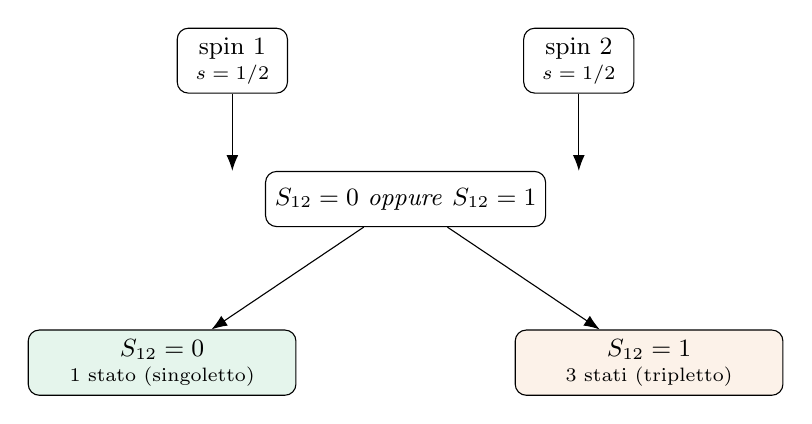
\begin{tikzpicture}[
  node distance=1.1cm,
  every node/.style={font=\small},
  leaf/.style={draw,rounded corners,minimum width=1.4cm,minimum height=0.7cm,align=center},
  box/.style={draw,rounded corners,minimum width=3.4cm,minimum height=0.7cm,align=center}
]
\node[leaf] (s1) at (-2.2,0) {spin 1\\[-2pt]{\scriptsize$s=1/2$}};
\node[leaf] (s2) at (2.2,0) {spin 2\\[-2pt]{\scriptsize$s=1/2$}};
\node[box,below=1.4cm of $(s1)!0.5!(s2)$] (comb) {$S_{12}=0$ \emph{oppure} $S_{12}=1$};
\draw[-{Latex[length=2mm]}] (s1) -- (comb.north -| s1);
\draw[-{Latex[length=2mm]}] (s2) -- (comb.north -| s2);
\node[box,below left=1.3cm and -0.4cm of comb,fill=colC!12] (S0) {$S_{12}=0$\\[-2pt]{\scriptsize 1 stato (singoletto)}};
\node[box,below right=1.3cm and -0.4cm of comb,fill=colA!10] (S1) {$S_{12}=1$\\[-2pt]{\scriptsize 3 stati (tripletto)}};
\draw[-{Latex[length=2mm]}] (comb) -- (S0);
\draw[-{Latex[length=2mm]}] (comb) -- (S1);
\end{tikzpicture}
\captionof{figure}{Passo 1: composizione dei due spin della coppia base. Dimensione totale $2\times2=4=1+3$: verificata.}
\label{fig:step1}
\end{center}

\section{Passo 2 — comporre $S_{12}$ con lo spin del sito 3}

\subsection{Quanti multipletti ci si aspetta, e perché}

Il conteggio dimensionale è il primo controllo, prima di ogni calcolo:
lo spazio di Hilbert a 3 qubit ha dimensione $2^3=8$. Dal Passo~1 sappiamo che
si divide in un settore $S_{12}=0$ (dimensione 1) e uno $S_{12}=1$ (dimensione 3);
componendo ciascuno con il terzo spin ($2^1=2$ stati), si ottiene $1\times2=2$
dal primo settore e $3\times2=6$ dal secondo, per un totale $2+6=8$ — coerente.

La regola generale di composizione di due momenti angolari $j_1,j_2$ dà
$S\in\{|j_1-j_2|,\dots,j_1+j_2\}$, ciascuno una volta sola. Qui $j_1=S_{12}=1$,
$j_2=\tfrac12$ (il sito 3): $S\in\{\tfrac12,\tfrac32\}$. Dimensioni: $S=3/2$
porta $2S{+}1=4$ stati, $S=1/2$ ne porta $2$: $4+2=6$, di nuovo coerente col
conteggio sopra. Sono i blocchi $A$ ($S=3/2$) e $B$ ($S=1/2$) della teoria.
Il settore $S_{12}=0$ (spin nullo) composto con $j_2=1/2$ dà banalmente
$S=1/2$ soltanto — un solo modo, nessuna scelta: è il blocco $C$.

\subsection{Blocco $A$ ($S=3/2$): costruzione via operatore di abbassamento}

\paragraph{Stato di partenza (banale).} C'è un solo modo di avere $M$ massimo:
tutti e tre gli spin "su". Nessuna sovrapposizione è possibile — è automaticamente
un autostato di $\mathbf S^2$:
\begin{equation}
\ket{A,{+}\tfrac32} = \ket{S_{12}{=}1,M_{12}{=}{+}1}\otimes\ket0_3 = \ket{00}\otimes\ket0_3 = \ket{000}.
\end{equation}

\paragraph{Operatore di abbassamento totale.} $S_-=S_{12,-}+s_{3,-}$, dove
$S_{12,-}$ agisce solo sul settore $S_{12}=1$ (tripletto) come operatore di
spin-1, e $s_{3,-}$ come operatore di spin-$\tfrac12$ sul terzo qubit. Usiamo
il risultato standard di teoria del momento angolare (non ridimostrato qui,
è algebra generale di $\mathfrak{su}(2)$):
\begin{equation}
S_-\ket{S,M} = \sqrt{S(S{+}1)-M(M{-}1)}\;\ket{S,M{-}1}.
\label{eq:ladder}
\end{equation}
Per il tripletto ($S_{12}=1$): $S_{12,-}\ket{1,{+}1}=\sqrt2\,\ket{1,0}$,
$S_{12,-}\ket{1,0}=\sqrt2\,\ket{1,{-}1}$, $S_{12,-}\ket{1,{-}1}=0$.
Per il terzo qubit: $s_{3,-}\ket0_3=\ket1_3$, $s_{3,-}\ket1_3=0$.

\paragraph{Primo passo: da $M{=}3/2$ a $M{=}1/2$.} Dall'eq.~\eqref{eq:ladder}
con $S=3/2,M=3/2$: coefficiente $\sqrt{\tfrac{15}{4}-\tfrac32\cdot\tfrac12}=\sqrt3$.
Applichiamo $S_-$ al vettore esplicito:
\begin{align*}
S_-\ket{000} &= \big(S_{12,-}\ket{00}\big)\otimes\ket0_3 + \ket{00}\otimes\big(s_{3,-}\ket0_3\big)\\
&= \sqrt2\,\ket{1,0}_{12}\otimes\ket0_3 + \ket{00}\otimes\ket1_3\\
&= \sqrt2\cdot\tfrac{1}{\sqrt2}(\ket{01}+\ket{10})\otimes\ket0_3 + \ket{001}\\
&= \ket{010}+\ket{100}+\ket{001}.
\end{align*}
Dividendo per $\sqrt3$ (normalizzazione del passo dell'eq.~\eqref{eq:ladder}):
\begin{equation}
\ket{A,{+}\tfrac12} = \tfrac{1}{\sqrt3}\big(\ket{001}+\ket{010}+\ket{100}\big).
\label{eq:Ap12}
\end{equation}
\emph{Verifica di consistenza:} il coefficiente della formula \eqref{eq:ladder}
dava $\sqrt3$ e infatti $\|\ket{010}+\ket{100}+\ket{001}\|=\sqrt3$ — il calcolo
esplicito e la formula generale coincidono, come devono.

\paragraph{Secondo passo: da $M{=}1/2$ a $M{=}{-}1/2$.} Formula: coefficiente
$\sqrt{\tfrac{15}{4}-\tfrac12\cdot({-}\tfrac12)}=\sqrt{4}=2$. Applichiamo $S_-$
di nuovo, questa volta termine per termine su ciascuno dei tre addendi di
$\sqrt3\,\ket{A,+\tfrac12}=\ket{001}+\ket{010}+\ket{100}$ (usando la
regola di Leibniz $S_-(u\otimes v)=(S_{12,-}u)\otimes v+u\otimes(s_{3,-}v)$
sito per sito):
\begin{align*}
S_-\ket{001} &= S_{12,-}\ket{00}\otimes\ket1_3 + \ket{00}\otimes s_{3,-}\ket1_3
= \sqrt2\,\tfrac{1}{\sqrt2}(\ket{01}{+}\ket{10})\ket1_3 + 0
= \ket{011}+\ket{101},\\
S_-\ket{010} &= S_{12,-}\ket{01}\otimes\ket0_3 + \ket{01}\otimes s_{3,-}\ket0_3.
\end{align*}
Qui serve l'azione di $S_{12,-}$ non su $\ket{1,M_{12}}$ direttamente ma sulla
combinazione: scriviamo $\ket{01}=\tfrac1{\sqrt2}(\ket{1,0}_{12}+\ket{S_{12}=0})$
(proiezione sui due settori) — ma poiché stiamo lavorando \emph{dentro} il
sottospazio $S_{12}=1$ (il blocco $A$ vive lì per costruzione), conviene
sommare direttamente $\ket{010}+\ket{100}=\sqrt2\,\ket{1,0}_{12}\otimes\ket0_3$
\emph{prima} di applicare $S_-$, invece di trattare i due termini separatamente:
\begin{align*}
S_-\big(\ket{010}+\ket{100}\big) &= \sqrt2\,S_-\big(\ket{1,0}_{12}\otimes\ket0_3\big)\\
&= \sqrt2\Big[\big(S_{12,-}\ket{1,0}_{12}\big)\otimes\ket0_3 + \ket{1,0}_{12}\otimes\big(s_{3,-}\ket0_3\big)\Big]\\
&= \sqrt2\Big[\sqrt2\,\ket{1,{-}1}_{12}\otimes\ket0_3 + \ket{1,0}_{12}\otimes\ket1_3\Big]\\
&= 2\,\ket{11}\otimes\ket0_3 + \sqrt2\cdot\tfrac{1}{\sqrt2}(\ket{01}{+}\ket{10})\otimes\ket1_3\\
&= 2\,\ket{110} + \ket{011}+\ket{101}.
\end{align*}
Sommando i due contributi calcolati ($S_-\ket{001}$ e $S_-(\ket{010}+\ket{100})$):
\begin{equation*}
S_-\big(\ket{001}+\ket{010}+\ket{100}\big) = (\ket{011}+\ket{101}) + \big(2\ket{110}+\ket{011}+\ket{101}\big)
= 2\big(\ket{011}+\ket{101}+\ket{110}\big).
\end{equation*}
Dividendo per il fattore $\sqrt3$ già raccolto a sinistra e per il coefficiente
$2$ della formula \eqref{eq:ladder}:
\begin{equation}
\ket{A,{-}\tfrac12} = \tfrac{1}{\sqrt3}\big(\ket{011}+\ket{101}+\ket{110}\big).
\label{eq:Am12}
\end{equation}

\paragraph{Ultimo passo: $M{=}{-}3/2$.} Per lo stesso argomento del primo
passo (un solo termine possibile, tutti gli spin "giù"), senza bisogno di
ricalcolare:
\begin{equation}
\ket{A,{-}\tfrac32} = \ket{111}.
\end{equation}

\subsection{Blocco $B$ ($S=1/2$, $S_{12}=1$): stati ortogonali ad $A$}

Nel settore $M=+\tfrac12$ (dimensione 2, generato da $\ket{001}$ e
$\tfrac{1}{\sqrt2}(\ket{010}+\ket{100})$, entrambi con $S_{12}=1$), l'eq.~\eqref{eq:Ap12}
si scrive nella base ortonormale $\{e_1,e_2\}\equiv\{\ket{001},\ \tfrac1{\sqrt2}(\ket{010}{+}\ket{100})\}$
come
\begin{equation}
\ket{A,{+}\tfrac12} = \tfrac{1}{\sqrt3}\,e_1 + \sqrt{\tfrac23}\,e_2 .
\end{equation}
(Verifica: $\tfrac1{\sqrt3}e_1+\sqrt{\tfrac23}e_2 = \tfrac1{\sqrt3}\ket{001}+\sqrt{\tfrac23}\cdot\tfrac1{\sqrt2}(\ket{010}{+}\ket{100})=\tfrac1{\sqrt3}(\ket{001}{+}\ket{010}{+}\ket{100})$ — coincide con l'eq.~\eqref{eq:Ap12}.)
Il vettore \emph{ortogonale} a $(\tfrac1{\sqrt3},\sqrt{\tfrac23})$ nel piano
reale $(e_1,e_2)$ è, a meno di fase globale, $(\sqrt{\tfrac23},-\tfrac1{\sqrt3})$:
\begin{equation}
\ket{B,{+}\tfrac12} = \sqrt{\tfrac23}\,e_1 - \tfrac{1}{\sqrt3}\,e_2
= \sqrt{\tfrac23}\,\ket{001} - \tfrac{1}{\sqrt6}\big(\ket{010}+\ket{100}\big).
\label{eq:Bp12}
\end{equation}
Questo \emph{deve} essere anche autostato di $\mathbf S^2$ con $S=1/2$ (non
serve verificarlo a parte: è garantito dal fatto che $\mathbf S^2$ è
un operatore hermitiano che commuta con $S_z$, quindi è diagonale a blocchi
in ciascun settore di $M$ fissato — un vettore ortogonale, in quel settore, a
un autovettore con autovalore diverso ($S{=}3/2$) è automaticamente autovettore
dell'autovalore complementare).

Lo stesso argomento nel settore $M=-\tfrac12$ (base $\{\ket{110},\ \tfrac1{\sqrt2}(\ket{011}{+}\ket{101})\}$,
con l'eq.~\eqref{eq:Am12} che si scrive $\ket{A,-\tfrac12}=\sqrt{\tfrac23}\,\tfrac1{\sqrt2}(\ket{011}{+}\ket{101})+\tfrac1{\sqrt3}\ket{110}$) dà, per ortogonalità:
\begin{equation}
\ket{B,{-}\tfrac12} = \tfrac{1}{\sqrt6}\big(\ket{011}+\ket{101}\big) - \sqrt{\tfrac23}\,\ket{110}.
\label{eq:Bm12}
\end{equation}

\begin{center}
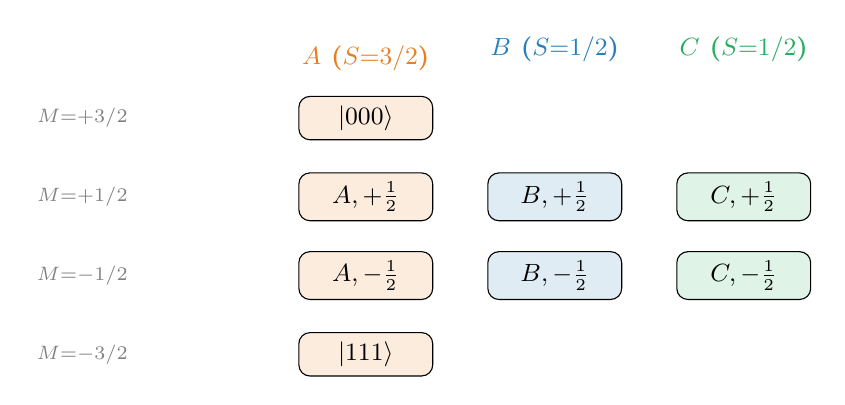
\begin{tikzpicture}[
  every node/.style={font=\small},
  M/.style={font=\scriptsize,gray}
]
\def\x{2.4}
\node[M] at (-3.6,1.5) {$M{=}{+}3/2$};
\node[M] at (-3.6,0.5) {$M{=}{+}1/2$};
\node[M] at (-3.6,-0.5) {$M{=}{-}1/2$};
\node[M] at (-3.6,-1.5) {$M{=}{-}3/2$};

\node[draw,rounded corners,fill=colA!15,minimum width=1.7cm] (a32) at (0,1.5) {$\ket{000}$};
\node[draw,rounded corners,fill=colA!15,minimum width=1.7cm] (a12) at (0,0.5) {$A,{+}\tfrac12$};
\node[draw,rounded corners,fill=colA!15,minimum width=1.7cm] (am12) at (0,-0.5) {$A,{-}\tfrac12$};
\node[draw,rounded corners,fill=colA!15,minimum width=1.7cm] (am32) at (0,-1.5) {$\ket{111}$};

\node[draw,rounded corners,fill=colB!15,minimum width=1.7cm] (b12) at (\x,0.5) {$B,{+}\tfrac12$};
\node[draw,rounded corners,fill=colB!15,minimum width=1.7cm] (bm12) at (\x,-0.5) {$B,{-}\tfrac12$};

\node[draw,rounded corners,fill=colC!15,minimum width=1.7cm] (c12) at (2*\x,0.5) {$C,{+}\tfrac12$};
\node[draw,rounded corners,fill=colC!15,minimum width=1.7cm] (cm12) at (2*\x,-0.5) {$C,{-}\tfrac12$};

\node[above=0.2cm of a32,font=\bfseries\small,colA] {$A$ ($S{=}3/2$)};
\node[above=1.28cm of b12,font=\bfseries\small,colB] {$B$ ($S{=}1/2$)};
\node[above=1.28cm of c12,font=\bfseries\small,colC] {$C$ ($S{=}1/2$)};
\end{tikzpicture}
\captionof{figure}{Diagramma dei livelli in $M$ per i tre blocchi. $A$ occupa i quattro valori $M=\pm3/2,\pm1/2$; $B$ e $C$, entrambi $S=1/2$, occupano solo $M=\pm1/2$ ma sono stati fisicamente distinti (diverso $S_{12}$, diversa energia — vedi teoria).}
\label{fig:levels}
\end{center}

\subsection{Blocco $C$ ($S_{12}=0$): il caso banale}

Con $S_{12}=0$ non c'è alcuna scelta: comporre spin $0$ con spin $\tfrac12$ dà
un solo multipletto, $S=\tfrac12$, e il terzo qubit resta ``spettatore''
inerte (nessun coefficiente di Clebsch–Gordan non banale, perché non c'è
degenerazione da risolvere):
\begin{align}
\ket{C,{+}\tfrac12} &= \ket{S_{12}{=}0}\otimes\ket0_3 = \tfrac{1}{\sqrt2}\big(\ket{010}-\ket{100}\big),\\
\ket{C,{-}\tfrac12} &= \ket{S_{12}{=}0}\otimes\ket1_3 = \tfrac{1}{\sqrt2}\big(\ket{011}-\ket{101}\big).
\end{align}

\section{Riepilogo e verifica numerica}

\begin{table}[h]
\centering
\renewcommand{\arraystretch}{1.5}
\begin{tabular}{@{}cccl@{}}
\toprule
Blocco & $S$ & $M$ & Stato esplicito \\
\midrule
\rowcolor{colA!8} $A$ & $3/2$ & $+3/2$ & $\ket{000}$\\
\rowcolor{colA!8} $A$ & $3/2$ & $+1/2$ & $\tfrac{1}{\sqrt3}(\ket{001}+\ket{010}+\ket{100})$\\
\rowcolor{colA!8} $A$ & $3/2$ & $-1/2$ & $\tfrac{1}{\sqrt3}(\ket{011}+\ket{101}+\ket{110})$\\
\rowcolor{colA!8} $A$ & $3/2$ & $-3/2$ & $\ket{111}$\\
\rowcolor{colB!8} $B$ & $1/2$ & $+1/2$ & $\sqrt{\tfrac23}\ket{001}-\tfrac{1}{\sqrt6}(\ket{010}+\ket{100})$\\
\rowcolor{colB!8} $B$ & $1/2$ & $-1/2$ & $\tfrac{1}{\sqrt6}(\ket{011}+\ket{101})-\sqrt{\tfrac23}\ket{110}$\\
\rowcolor{colC!8} $C$ & $1/2$ & $+1/2$ & $\tfrac{1}{\sqrt2}(\ket{010}-\ket{100})$\\
\rowcolor{colC!8} $C$ & $1/2$ & $-1/2$ & $\tfrac{1}{\sqrt2}(\ket{011}-\ket{101})$\\
\bottomrule
\end{tabular}
\caption{Gli otto stati derivati, in base computazionale $\ket{q_1q_2q_3}$.}
\label{tab:stati}
\end{table}

\paragraph{Verifica indipendente (autotest numerico).} Coerentemente con la
convenzione di autotest a precisione macchina già seguita nel resto del
progetto, questi otto vettori sono stati verificati con \texttt{NumPy} contro
$H$ dell'eq.~\eqref{eq:H} scritta in convenzione di Pauli diretta (stessa
funzione \texttt{H\_trimero} di \texttt{verifica.py}), a un punto
$(J,J',b)=(1.3,-0.7,0.9)$ scelto casualmente (nessuna simmetria accidentale
che potrebbe mascherare un errore):
\begin{center}
\small
\begin{tabular}{lccc}
\toprule
Stato & $\lVert\psi\rVert^2$ & $E_\text{num}=\bra\psi H\ket\psi$ & $E_\text{teorico}=E(S_{12},S)+2bM$\\
\midrule
$A,{+}3/2$ & $1.000000000000$ & $2.60000$ & $2.60000$ \\
$A,{+}1/2$ & $1.000000000000$ & $0.80000$ & $0.80000$ \\
$A,{-}1/2$ & $1.000000000000$ & $-1.00000$ & $-1.00000$ \\
$A,{-}3/2$ & $1.000000000000$ & $-2.80000$ & $-2.80000$ \\
$B,{+}1/2$ & $1.000000000000$ & $5.00000$ & $5.00000$ \\
$B,{-}1/2$ & $1.000000000000$ & $3.20000$ & $3.20000$ \\
$C,{+}1/2$ & $1.000000000000$ & $-3.00000$ & $-3.00000$ \\
$C,{-}1/2$ & $1.000000000000$ & $-4.80000$ & $-4.80000$ \\
\bottomrule
\end{tabular}
\end{center}
Errore massimo su energia: $8.9\times10^{-16}$; errore massimo su norma:
$2.2\times10^{-16}$; massimo elemento fuori diagonale della matrice di Gram
(ortogonalità reciproca dei vettori): $6.7\times10^{-17}$ — tutti a
precisione macchina, nessuna discrepanza fisica. Inoltre, per ciascuno stato
è stato verificato $\lVert H\ket\psi - E_\text{teorico}\ket\psi\rVert\sim10^{-16}$:
sono autovettori \emph{esatti}, non solo a valore d'aspettazione corretto.

\section{Struttura degli stati: cosa significa per la preparazione su circuito}

\begin{center}
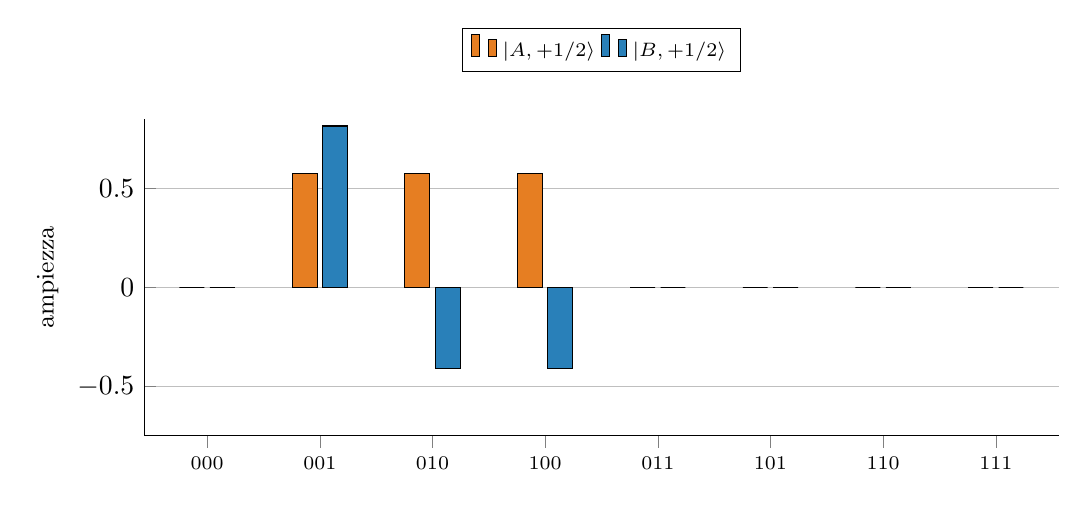
\begin{tikzpicture}
\begin{axis}[
  ybar,
  bar width=9pt,
  width=13.2cm, height=5.6cm,
  symbolic x coords={000,001,010,100,011,101,110,111},
  xtick=data,
  x tick label style={font=\scriptsize},
  ylabel={ampiezza},
  ylabel style={font=\small},
  ymin=-0.75, ymax=0.85,
  legend style={font=\scriptsize,at={(0.5,1.15)},anchor=south,legend columns=3},
  enlarge x limits=0.08,
  axis lines*=left,
  ymajorgrids,
  clip=false
]
\addplot[fill=colA] coordinates {
  (000,0) (001,0.5774) (010,0.5774) (100,0.5774) (011,0) (101,0) (110,0) (111,0)
};
\addplot[fill=colB] coordinates {
  (000,0) (001,0.8165) (010,-0.4082) (100,-0.4082) (011,0) (101,0) (110,0) (111,0)
};
\legend{$\ket{A,+1/2}$,$\ket{B,+1/2}$}
\end{axis}
\end{tikzpicture}
\captionof{figure}{Ampiezze (reali) di $\ket{A,{+}1/2}$ e $\ket{B,{+}1/2}$ sugli stessi tre stati computazionali. Stesso \emph{supporto} (i termini non nulli coincidono), ma pesi e segno relativo diversi: $A$ è la sovrapposizione simmetrica ``stato-W'' a coefficienti uguali; $B$ pesa doppiamente lo stato isolato $\ket{001}$ e con segno opposto gli altri due.}
\label{fig:amplitudes}
\end{center}

\begin{table}[h]
\centering
\renewcommand{\arraystretch}{1.3}
\begin{tabular}{@{}lll@{}}
\toprule
Stato & Struttura & Preparazione\\
\midrule
$\ket{C,\pm\tfrac12}$ & prodotto singoletto$_{12}\otimes\ket{\cdot}_3$ & \textbf{banale}: identico al singoletto del dimero\\
 & & ($X,H,\mathrm{CNOT},X$ su 1,2) $+$ eventuale $X$ su 3\\
$\ket{A,\pm\tfrac32}$ & stato prodotto puro & \textbf{banale}: solo porte $X$\\
$\ket{A,\pm\tfrac12}$ & sovrapposizione a 3 termini, & \textbf{non banale}: stato di tipo W,\\
 & pesi uguali (stato W) & serve una sequenza di rotazioni controllate\\
$\ket{B,\pm\tfrac12}$ & sovrapposizione a 3 termini, & \textbf{non banale}: stessa famiglia di $A_{1/2}$\\
 & pesi $2{:}1{:}1$ e segno relativo & ma pesi/segni diversi\\
\bottomrule
\end{tabular}
\caption{Complessità di preparazione dei diversi stati.}
\label{tab:prep}
\end{table}

\section{Collegamento con il punto di lavoro proposto}

Per il punto di test $(J,J')=(1,0.4)$ (regione C della mappa dei segni,
$b_c=2.4$), a campo $0<b<b_c$ il fondamentale è $\ket{C,{-}\tfrac12}$: proprio
lo stato più semplice della Tabella~\ref{tab:prep}, identico (a meno di una
$X$ sul terzo qubit) al singoletto già usato come stato iniziale del PMA per
il dimero. È coerente con la scelta di partire da questo punto per il primo
test end-to-end del VQE a 3 qubit: nessun circuito di preparazione nuovo da
sviluppare per lo stato iniziale. Gli stati di tipo W ($A_{\pm1/2}$, $B_{\pm1/2}$)
resteranno necessari solo se in futuro si esplora un punto in regione B, o si
scansiona attraverso $b_c$ entrando nel blocco $A$.

\section*{Appendice — riepilogo delle formule}
\begin{align*}
\ket{S_{12}{=}0} &= \tfrac1{\sqrt2}(\ket{01}-\ket{10}) &
\ket{S_{12}{=}1,0} &= \tfrac1{\sqrt2}(\ket{01}+\ket{10})\\
\ket{A,{+}\tfrac32} &= \ket{000},\quad \ket{A,{-}\tfrac32}=\ket{111} &
\ket{A,{+}\tfrac12} &= \tfrac1{\sqrt3}\big(\ket{001}{+}\ket{010}{+}\ket{100}\big) \\
& &
\ket{A,{-}\tfrac12} &= \tfrac1{\sqrt3}\big(\ket{011}{+}\ket{101}{+}\ket{110}\big) \\
\ket{B,{+}\tfrac12} &= \sqrt{\tfrac23}\ket{001}-\tfrac1{\sqrt6}(\ket{010}{+}\ket{100}) &
\ket{B,{-}\tfrac12} &= \tfrac1{\sqrt6}(\ket{011}{+}\ket{101})-\sqrt{\tfrac23}\ket{110}\\
\ket{C,{+}\tfrac12} &= \tfrac1{\sqrt2}(\ket{010}-\ket{100}) &
\ket{C,{-}\tfrac12} &= \tfrac1{\sqrt2}(\ket{011}-\ket{101})
\end{align*}
Operatore di abbassamento usato: $S_-\ket{S,M}=\sqrt{S(S{+}1)-M(M{-}1)}\,\ket{S,M{-}1}$
(risultato standard dell'algebra $\mathfrak{su}(2)$, non ridimostrato).

\end{document}
